% Scaling functions (basis) for V_3: eight piecewise constant functions
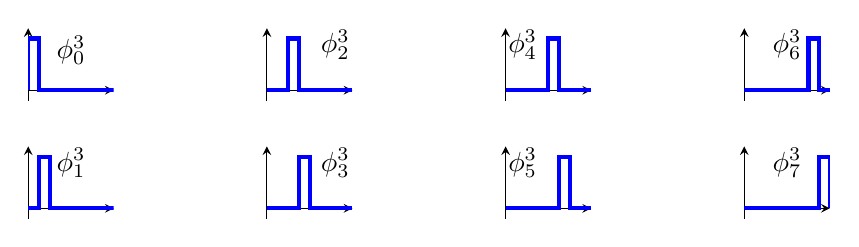
\begin{tikzpicture}
  % Column 1: Scaling functions 1 and 2
  % Scaling function 1: [0, 1/8)
  \begin{axis}[
    at={(0,0)},
    width=0.22\textwidth,
    height=2.5cm,
    xmin=0, xmax=1,
    ymin=-0.2, ymax=1.2,
    ytick=\empty,
    xtick=\empty,
    axis x line=middle,
    axis y line=center,
  ]
    \addplot[const plot, line width=1.5pt, color=blue] coordinates {
      (0,0) (0,1) (0.125,1) (0.125,0) (1,0)
    };
    \node[above] at (0.5, 0.3) {$\phi_0^3$};
  \end{axis}
  % Scaling function 2: [1/8, 1/4)
  \begin{axis}[
    at={(0,-1.5cm)},
    width=0.22\textwidth,
    height=2.5cm,
    xmin=0, xmax=1,
    ymin=-0.2, ymax=1.2,
    ytick=\empty,
    xtick=\empty,
    axis x line=middle,
    axis y line=center,
  ]
    \addplot[const plot, line width=1.5pt, color=blue] coordinates {
      (0,0) (0.125,0) (0.125,1) (0.25,1) (0.25,0) (1,0)
    };
    \node[above] at (0.5, 0.4) {$\phi_1^3$};
  \end{axis}
  
  % Column 2: Scaling functions 3 and 4
  % Scaling function 3: [1/4, 3/8)
  \begin{axis}[
    at={(0.25\textwidth,0)},
    width=0.22\textwidth,
    height=2.5cm,
    xmin=0, xmax=1,
    ymin=-0.2, ymax=1.2,
    ytick=\empty,
    xtick=\empty,
    axis x line=middle,
    axis y line=center,
  ]
    \addplot[const plot, line width=1.5pt, color=blue] coordinates {
      (0,0) (0.25,0) (0.25,1) (0.375,1) (0.375,0) (1,0)
    };
    \node[above] at (0.8, 0.4) {$\phi_2^3$};
  \end{axis}
  % Scaling function 4: [3/8, 1/2)
  \begin{axis}[
    at={(0.25\textwidth,-1.5cm)},
    width=0.22\textwidth,
    height=2.5cm,
    xmin=0, xmax=1,
    ymin=-0.2, ymax=1.2,
    ytick=\empty,
    xtick=\empty,
    axis x line=middle,
    axis y line=center,
  ]
    \addplot[const plot, line width=1.5pt, color=blue] coordinates {
      (0,0) (0.375,0) (0.375,1) (0.5,1) (0.5,0) (1,0)
    };
    \node[above] at (0.8, 0.4) {$\phi_3^3$};
  \end{axis}
  
  % Column 3: Scaling functions 5 and 6
  % Scaling function 5: [1/2, 5/8)
  \begin{axis}[
    at={(0.5\textwidth,0)},
    width=0.22\textwidth,
    height=2.5cm,
    xmin=0, xmax=1,
    ymin=-0.2, ymax=1.2,
    ytick=\empty,
    xtick=\empty,
    axis x line=middle,
    axis y line=center,
  ]
    \addplot[const plot, line width=1.5pt, color=blue] coordinates {
      (0,0) (0.5,0) (0.5,1) (0.625,1) (0.625,0) (1,0)
    };
    \node[above] at (0.2, 0.4) {$\phi_4^3$};
  \end{axis}
  % Scaling function 6: [5/8, 3/4)
  \begin{axis}[
    at={(0.5\textwidth,-1.5cm)},
    width=0.22\textwidth,
    height=2.5cm,
    xmin=0, xmax=1,
    ymin=-0.2, ymax=1.2,
    ytick=\empty,
    xtick=\empty,
    axis x line=middle,
    axis y line=center,
  ]
    \addplot[const plot, line width=1.5pt, color=blue] coordinates {
      (0,0) (0.625,0) (0.625,1) (0.75,1) (0.75,0) (1,0)
    };
    \node[above] at (0.2, 0.4) {$\phi_5^3$};
  \end{axis}
  
  % Column 4: Scaling functions 7 and 8
  % Scaling function 7: [3/4, 7/8)
  \begin{axis}[
    at={(0.75\textwidth,0)},
    width=0.22\textwidth,
    height=2.5cm,
    xmin=0, xmax=1,
    ymin=-0.2, ymax=1.2,
    ytick=\empty,
    xtick=\empty,
    axis x line=middle,
    axis y line=center,
  ]
    \addplot[const plot, line width=1.5pt, color=blue] coordinates {
      (0,0) (0.75,0) (0.75,1) (0.875,1) (0.875,0) (1,0)
    };
    \node[above] at (0.5, 0.4) {$\phi_6^3$};
  \end{axis}
  % Scaling function 8: [7/8, 1)
  \begin{axis}[
    at={(0.75\textwidth,-1.5cm)},
    width=0.22\textwidth,
    height=2.5cm,
    xmin=0, xmax=1,
    ymin=-0.2, ymax=1.2,
    ytick=\empty,
    xtick=\empty,
    axis x line=middle,
    axis y line=center,
  ]
    \addplot[const plot, line width=1.5pt, color=blue] coordinates {
      (0,0) (0.875,0) (0.875,1) (1,1) (1,0)
    };
    \node[above] at (0.5, 0.4) {$\phi_7^3$};
  \end{axis}
\end{tikzpicture}

